\section{Numerical climate modelling}
Climatology describes the statistical distribution of variables of interest at the Earth's surface and in the atmosphere, among which temperature, pressure, humidity, precipitation, and wind speed.
For centuries, it remained a field of science based on observations, followed by the formulation of conceptual models, physical interpretation of wind patterns \citep{Halley1686, Hadley1735, Dove1837, Ferrel1856} and mathematical representations of the energy balance and radiative tranfer processes \citep{edwards_history_2011}.
The motions of the atmosphere are largely driven by fluids mechanics, which can be described by the Navier-Stokes equations, derived in the 19th century. However these equations do not have any known analytical solution, which forbids their direct use to predict motions of air, water and other components of the atmosphere. 
Modern climate modelling originated in the 1950s with the development of computer simulations which enable numerically estimating solutions of these equations.

\subsection{From GCMs to ESMs}

\begin{figure}[hbtp]
    \centering
    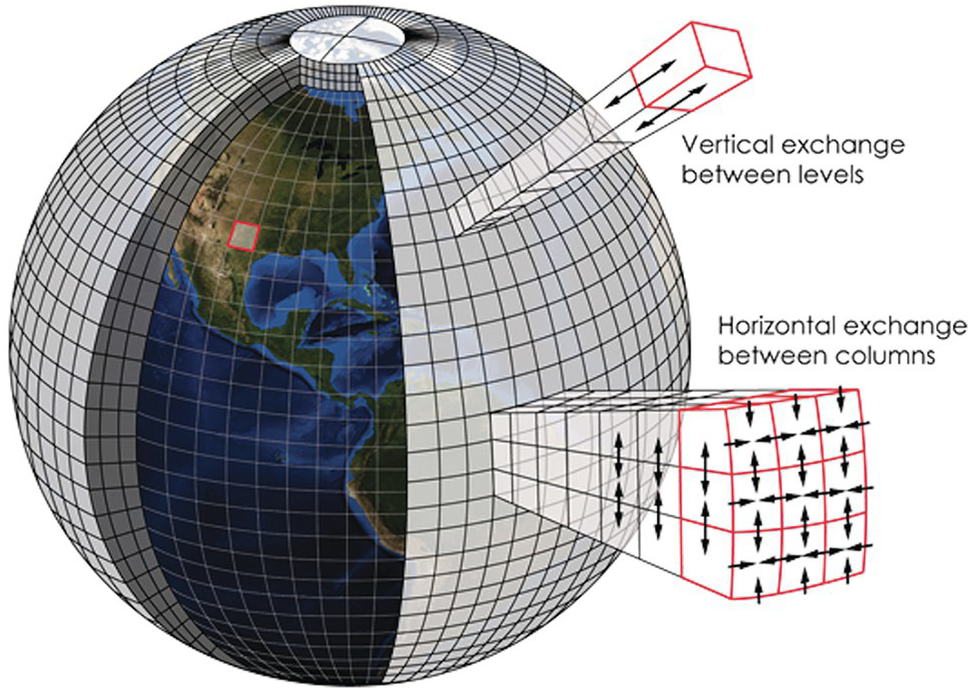
\includegraphics[width=0.7\textwidth]{images/intro/GCM_structure_kotamarthi.png}
    \caption{Representation of the structure of a GCM. Parametrizations apply to the vertical columns and the dynamics manages exchanges between columns. Taken from \citep{kotamarthi_downscaling_2021}. 
    }
    \label{fig:GCM}
\end{figure}

General circulation models (GCMs) use a simplified version of the Navier-Stokes equations, referred to as \textit{primitive equations} \citep[initially formulated in ][]{bjerknes1910}, to represent the complex motions of the atmosphere. 
The globe is discretized into grid cells, which can range from a few tens to a few hundreds of kilometers. Using an appropriate temporal discretization to account for Courant-Friedrichs-Lewy (CFL) conditions \citep{courant_partial_1967}, this enables approximating solutions of the primitive equations to represent atmospheric dynamics. This part of the GCM is often referred to as \textit{the dynamical core} or simply \textit{the dynamics} of the model. 
However, several major processes of the climate system are not described by fluid mechanics and require additional \textit{parametrizations}, which compute their average effect in each vertical column, independently of neighbouring grid cells. 
This part of the GCM is often referred to as \textit{the physics} of the model.
Most importantly, it represents all radiative emission and transfer processes, which largely dictate the energy budget of the atmosphere.
Thermodynamic processes involved in the phase changes of water are also essential to represent energy transfers between phases, cloud formation and precipitation. Parametrizations are also used to account for the processes that occur at a smaller scale than the resolution of the GCM and cannot be described by the dynamical core, such as turbulent diffusion or shallow and deep convection processes. Finally, parametrizations are used to represent interactions of the atmosphere with the various surfaces it can be interfaced with: sea surface, ice caps or sea ice, bare soil, vegetation, urban areas... 
Interactions between the land surface and the atmosphere and the feedback loops between the two systems are a major focus of this thesis, and Section \ref{sec:l-a_interactions} provides a detailed description of the state of knowledge in this field. 

Historically, the first climate models primarily focused on the atmosphere, with
a very simplified representation of the surface. Over the past three decades, climate models have evolved to distincly represent oceanic and continental surfaces by coupling atmospheric models with ocean models and land surface models (LSMs), and are now often referred to as Earth system models (ESMs). Nowadays, ESMs are not only used to simulate meteorological variables, but can have a much wider range of applications in geoscience, paleoclimatology, oceanography, glaciology, subsurface hydrology, biology, biogeochemistry, etc... (Fig. \ref{fig:GCM_processes}).
Regarding land surface in particular, the complexity of LSMs has gradually increased, for example, to better account for the influence of vegetation on the atmosphere, or to represent additional processes of interest such as rivers and groundwater, biogeochemical cycles of carbon or nitrogen, and anthropic activities like irrigation (which will be futher introduced in Section \ref{sec:irrig_context}). 

\begin{figure}[hbtp]
    \centering
    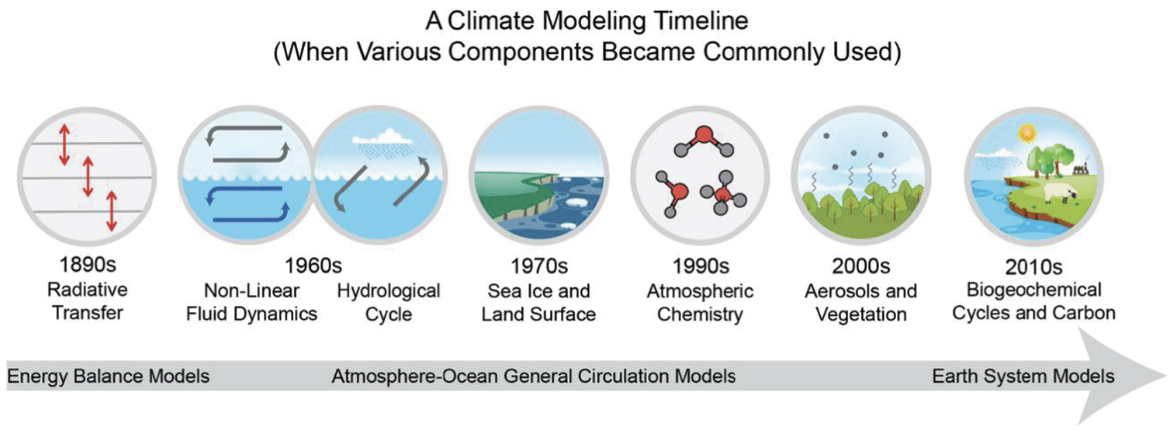
\includegraphics[width=0.9\textwidth]{images/intro/climate_modelling_evolution_kotamarthi.png}
    \caption{Gradual implementation of new processes in climate models. Taken from \citep{kotamarthi_downscaling_2021}. 
    }
    \label{fig:GCM_processes}
\end{figure}

A major limitation of GCMs and ocean models is computing power, which requires to balance the spatial and temporal resolution and the period covered by the simulation, to limit the actual time it will require to run on a given (super)computer. A given ESM can therefore be used in different setups, with coarse resolution to study paleoclimates over the last 10.000 years, or with finer resolution to analyze a specific process over the 21st century only. This means that model developers and users must be aware of the scale-dependent hypotheses and parameters introduced in the parametrizations to ensure that they remain suitable in different use cases.
It is also common to use the atmospheric GCM and LSM together but without coupling them to an ocean model, taking reference values for sea surface temperature instead (either from observations or previous fully-coupled simulations). Similarly, ocean models and LSMs can be run as standalone models using atmospheric forcings instead of a dynamical coupling with a GCM. 

Moreover, these constraints on computing power have also led to the development of other types of atmospheric models to lift some of the constraints on spatial resolution and address different goals, such as weather prediction or the study of specific processes. 

\subsection{A hierarchy of atmospheric models and scales}

Although they historically have and still share common developments, climate models must be distinguished from  Numerical Weather Prediction (NWP) models.
The physical systems and variables they aim to represent are the same, but the objectives are different, as climate models focus on interannual or even interdecadal averages, whereas NWP models try to predict precise weather conditions over a few days. 
Climate models therefore place emphasis on the correct representation of the mean state of climate and long-term feedbacks between various Earth system components (the atmosphere, oceans, land surface, and cryosphere).
Modern NWP, on the contrary, is expected to forecast and reproduce specific meteorological events, usually on a specific region as it is often conducted by national agencies. NWP models therefore simulate limited domains, which require realistic boundary conditions to take into account large-scale atmospheric features without having to explicitly simulate the global circulation. 
The predictions are also very dependent on the initial state of the model, which is rendered more realistic by the assimilation of observational data. Climate models do not have such a dependency as long as the initial state is generally representative of a stable state of the climate system. To ensure this, spinup or warmup runs are conducted before launching the actual simulation to reach a realistic state of equilibrium. They can last from a few months to hundreds of year depending on the processes studied.
%option:mention ensembles here ?

Another major difference between climate and NWP models is the resolution of the grid used. Climate models grid cells are usually a few tens of even a few hundreds of kilometer wide, wheareas NWP aims for higher spatial resolutions to provide localised forecasts. Many models currently operate at kilometer-scale resolutions, and the 100-meter scale is being investigated and considered for future deployments \citep{lean_hectometric_2024}.
As mentionned before, several scale-dependent hypotheses and parameters of climate models regarding the dynamics, the physics and their coupling, are not suitable at such resolutions. In particular, the scale separation between processes that are effectively resolved by the dynamics and processes that must be parametrized cannot be universal accross scales. For instance, when model resolution reaches the average size of a single cloud, statistical parametrizations of the cloud population then become partly inadapted, yet the dynamical core is not fully capable of properly representing their distribution. Multiple \textit{grey zones} are therefore identified for processes that were historically parametrized in atmospheric models, as scales within which new representations need to be developed \citep{wei_research_2024,frassoni_building_2018,chow_crossing_2019}.

Beyond the distinction between climate modelling and NWP, multiple types of atmospheric models exist, which can be used in different contexts.
Regional climate models are mostly based on the same structure and assumptions as global climate models but are used on limited area domains (typically a few hundred of kilometers), which lowers computational costs, but requires lateral boundary conditions.
The appellation \textit{mesoscale models} also covers this kind of domain \citep[mesoscale meteorological processes usually range from 10 to 200 km,][]{malardel2005fondamentaux}, but includes models with physical assumptions closer to NWP models that enable higher resolution.
Among these, multiple terms like storm-resolving, convection-permitting, or cloud-resolving models (CRMs) regroup models that explicitly represent convective clouds. They can be run at resolutions ranging from a few tens of metres to a few kilometres, and are usually based on non-hydrostatic physics.
As explained in a review of CRMs by \citet{guichard_short_2017}:
\begin{quote}
    ``CRMs are fine-scale limited-area numerical models whose major characteristic is to provide explicit simulations of the mesoscale dynamics associated with convective clouds. They integrate parametrizations in order to represent major sub-grid processes (turbulence, microphysics, radiative processes). However, unlike GCMs, their grid size allows numerous couplings arising between convective motions and physical processes to be resolved. [...] their utilization has proved very fruitful to the understanding of several convective cloud-related issues that cannot be satisfactorily addressed with observations alone; they are also now widely used as 'numerical laboratories' which guide and help the development of cloud and convection parametrizations for larger-scale models."
\end{quote}
Global CRMs have also been implemented, and although they cannot be used for long climate runs at the moment, they are expected to play an important role in the study and understanding of weather and climate in the future \citep{satoh_global_2019}.
At even finer resolution, down to the meter scale, are large eddy simulations (LES). They consist in a different class of models that achieve much higher performance on the representation of turbulent motions by using different assumptions to numerically approximate the Naver-Stokes equations. These models still filter some of the finer-scale motions and have their own parametrizations for these processes, but can be of great use for process understanding and to design parametrizations for mesoscale models or GCMs. 
Finally, the ultimate refinement of computational fluid dynamics is the use direct numerical simulations (DNS), which do not require any parameterization of turbulence, but are very demanding in computing power, and therefore limited to meter-scale domains and very short simulation periods.

To summarize, although not all approaches nor conceptual abstraction levels have been mentionned here, atmospheric modelling relies on a hierarchy of models which can support each other for both research and operational purposes \citep{maher_model_2019}. Larger models like ESMs can be used to provide boundary conditions for smaller ones at higher resolutions, which are in turn used to improve process understanding and parametrizations in coarser models.
These approaches have been particularly succesful at representing the state of climate, and at predicting climate change.

\subsection{Predicting climate change}
As early as 1824, Joseph Fourier, followed by Claude Pouillet, theorised that some components of the atmosphere can influence the temperature of the air more than others, which was demonstrated in 1838 by Eunice Newton Foote for water vapour and carbon dioxide (CO2). This was linked to infrared absorption and emissions by the experimental work of John Tyndall, and, in 1896, Svante Arrhenius conducted the first estimate of the global temperature increase caused by a hypothetical doubling of CO2 in the atmosphere \citep{tyndall_j_xxiii_1861, arrhenius_xxxi_1896}.
Since the industrial revolution in the 19th century, anthropic activities have increased the amounts of greenhouse gases in the atmosphere, mainly as a consequence of fossil fuel combustion and by destruction of natural sinks to give way to agricultural land \citep{RN1}.
By the end of the 1950s, it was established that concentration of CO2 in the atmosphere was increasing and monitoring efforts intensified \citep{pales_concentration_1965}.
Indeed, it was known that although water vapour is overwhelmingly dominant in the atmospheric composition, other greenhouse gases such as CO2, could have a significant impact on global energy balance, and therefore temperature, by absorbing infrared radiation in a different part of the spectrum \citep{plass_carbon_1956}.
Concurrent research in paleoclimatology showed that previous evolutions of greenhouse gases in the atmosphere had never been this fast, and were all associated with large-scale changes in global climate \citep{lorius_30000-yr_1979}.
At this time, concerns arose about the possible rise of global temperatures and the impacts it could have on natural ecosystems and human activities.\citep{broecker_climatic_1975}

As this knowledge progressed coincidentally with capablilities in numerical climate modelling, models started to be used not only to reproduce past and present climate, but also to simulate future climate scenarios. 
In particular, Syukuro Manabe simulated the impact of greenhouse gases on the thermal equilibrium of the atmosphere in single-column models \citep{manabe_thermal_1964}, before conducting groundbreaking work with coupled ocean-atmosphere GCMs to simulate the response of climate to an increase of atmospheric CO2 \citep{manabe_sensitivity_1980}. 
Such modelling experiments quickly confirmed the risk of rapid increases in global temperature, and hinted at the global and regional consequences on ice cap and glacier melting, sea level rise, and disruption of the water cycle, among others \citep{hansen_global_1988}. 
In 1988, the International Panel on Climate Change (IPCC) was established by the World Meteorological Organisation (WMO) and the United Nations Environment Program (UNEP) to unify efforts in climate change science, and on the socio-economic impacts of global warming. Since its first report \citep{IPCC_1990_AR1_WG1} the IPCC has been carrying on in its mission to "provide governments at all levels with scientific information that they can use to develop climate policies".

At the end of the 20th and the beginning of the 21st century, many developments in the field of remote sensing enabled the monitoring of climate variables from satellites, which complemented ground-based observations. This largely contributed to the ability to isolate the signal of anthropogenic climate change from natural climate variability in recent observations, retroactively validating climate change predictions established in the previous decades \citep{hansen_earths_2005,yang_role_2013}. 
In 2021, Syukuro Manabe shared one half of the Nobel Prize in Physics with Klaus Hasselmann "for the physical modelling of Earth's climate, quantifying variability and reliably predicting global warming". 
Hasselmann's work focused on the statistical methods that allowed to disentangle the variations in weather from long-term changes of climate induced by external forcings, such as anthropogenic grennhouse gases emissions, and identify a \textit{fingerprint} of climate change \citep{hasselmann_optimal_1993,hasselmann_stochastic_2022}.

Early studies focused on idealised scenarios, such as the doubling of atmospheric CO2, but the IPCC has since introduced a new standard for future climate simulations of different scenarios, to prepare its 6th Assessment Report \citep{RN1}. These Shared Socio-economic Pathways (SSPs) encompass different trajectories for population, economic development, education, and technological change to represent a range of plausible futures for human society. They are associated to Representative Concentration Pathways (RCPs), which quantify the additional radiative forcing on the global energy budget induced by greenhous gases emissions.
This approach allows climate modelers to assess a wide spectrum of scenarios, providing policymakers with a range of possible evolutions of the climate system (Fig. \ref{fig:ipcc_ssp}).

\begin{figure}[hbtp]
    \centering
    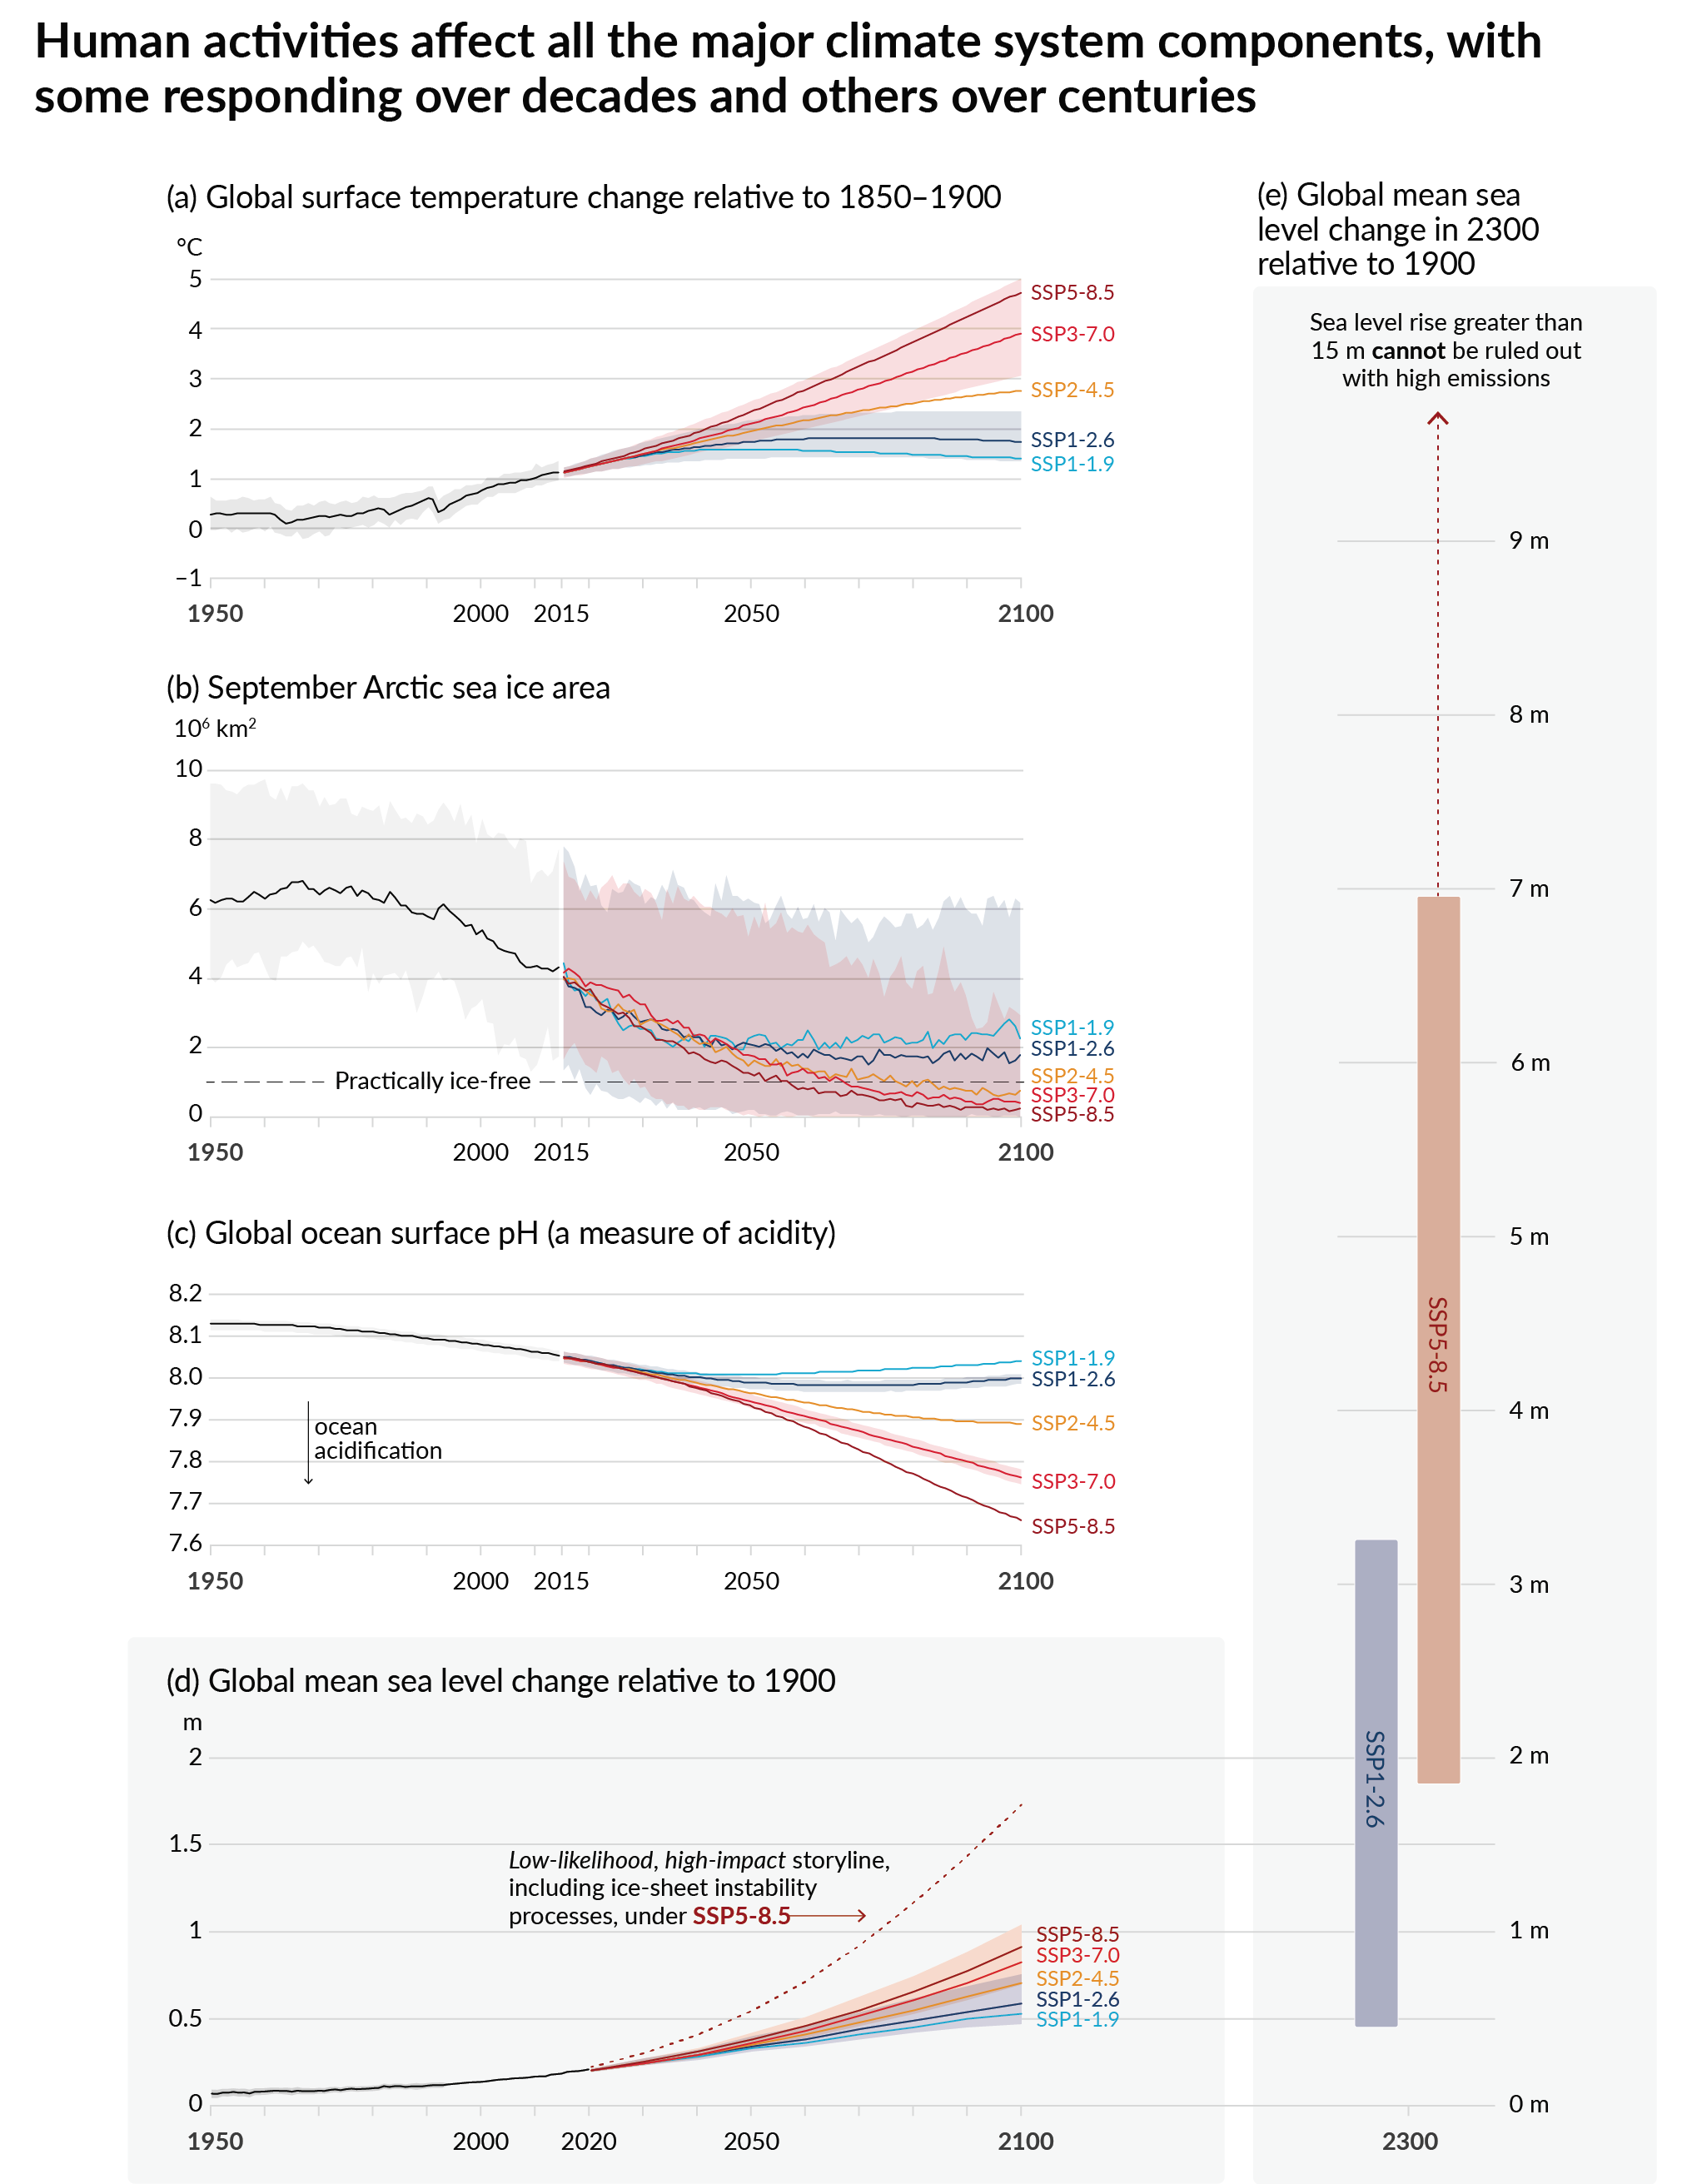
\includegraphics[width=\textwidth]{images/intro/IPCC_AR6_WGI_SPM_Figure_8.png}
    \caption{Selected indicators of global climate change under five scenarios used in the Summary for policymakers of the 6th Assessment Report \citep{IPCC_2023}.}
    \label{fig:ipcc_ssp}
\end{figure}

\clearpage

\section{Irrigation in the world and in the Iberian Peninsula}
\label{sec:irrig_context}
Irrigation is an ancestral agricultural practice which consists in providing additional water to cultivated soil to favor crop growth.
This practice is widespread globally in various forms and enables agriculture to maintain yields that would not be achievable in many regions otherwise \citep{siebert_quantifying_2010}.
Multiple techniques have been developed for irrigation, as a response to different contexts regarding available water quantities, technological developments, and the type of crops grown (Fig. \ref{fig:irrig_methods}).
Gravity irrigation, the most ancient method, is conducted by diverting surface water from natural sources or artifical storage reservoirs to the fields. In particular, flood irrigation methods cover entire fields with water, saturating the upper layers of the soil. It is rather simple to implement as it requires little infrastructure and technology, but remains largely inefficient as a large share of the water is evaporated without directly benefiting the crops.
Sprinkler irrigation achieves lower water consumption by spraying the water in the air above the fields, although part of it is intercepted by the leaves instead of directly reaching the soil and roots of crops, like natural rainfall. It requires more infrastructure to cover large surfaces and external energy to power the sprinklers.
Finally, drip irrigation uses pipes to provide smaller amounts of water directly at the base of the crops. If managed properly, this method has a much higher water use efficiency since it avoids both excessive runoff and evaporation of water. Its downside is that it requires a lot of equipment that has to be maintened to remain efficient, but that does not prevent this method from being increasingly used \citep{mpanga_decade_2021, pool_flood_2021}.

\begin{figure}[hbtp]
    \centering
    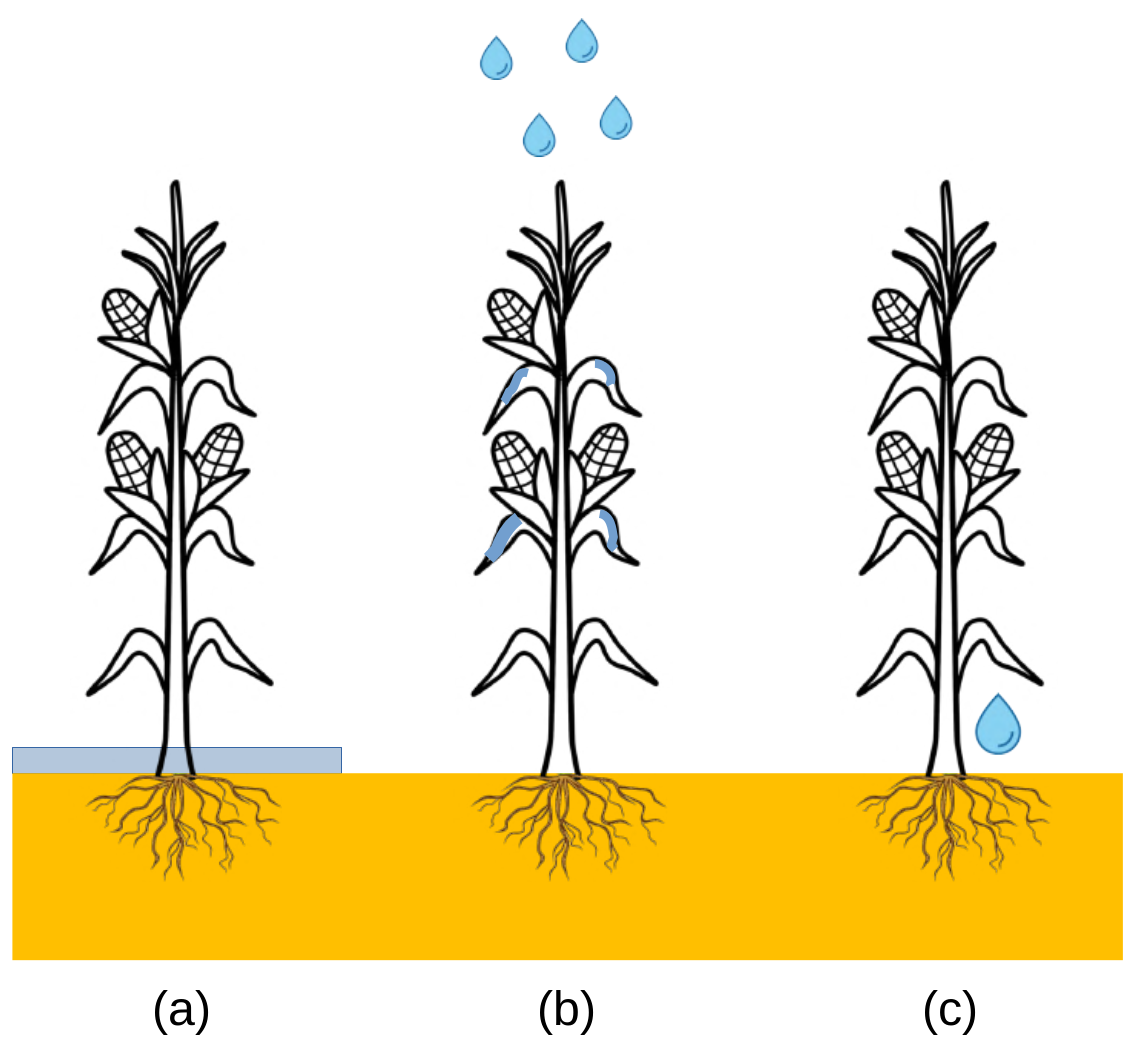
\includegraphics[width=0.7\textwidth]{images/intro/irrigation_methods_lunel.png}
    \caption{Schematic representation of the three main irrigation techniques: (a) flood irrigation, (b) sprinkler irrigation, and (c) drip irrigation. Taken from \citet{lunel_interactions_2024}.}
    \label{fig:irrig_methods}
\end{figure}

\subsection{The increasing use and impacts of irrigation}

Irrigated fields are estimated to cover about 20\% of global cropland (3.5 million km$^2$), which account for 40\% of the food produced in the world according to the United Nations Food and Agriculture Organization \citep{UNESCO2019,mcdermid_irrigation_2023}.
The historical reconstruction by \citet{siebert_global_2015} estimates that the total irrigated area increased fivefold during the 20th century due to population growth and industrialization, rising from 63 Mha in 1900 to 306 Mha in 2005. Certain regions stand out, such as South Asia, the Western United States of America (USA), Eastern China, and Western Europe (Figure \ref{irrig_evolution_map}).
This trend has continued in the 21st century, with an 11\% increase in irrigated areas from 2000 (297 Mha) to 2015 (330 Mha) according to \citet{mehta_half_2024}, which insisted on the fact that at least half of this expansion occured in water-stressed regions, raising concerns over sustainalility.
In the future, irrigation demand is projected to keep rising in most scenarios, especially during the summer in the Northern Hemisphere as a consequence of climate change \citep{wada_multimodel_2013,busschaert_net_2022}. 

\begin{figure}[ht]
    \centering
    
\includegraphics[width=\textwidth]{images/intro/irrig_evolution_Siebert.png}
    \caption{Percentage of area equipped for irrigation in 1900, 1960, and 2005 according to the Historical Irrigation Dataset (HID). Taken from \citet{siebert_global_2015}.}
    \label{irrig_evolution_map}
\end{figure}

Irrigation already has a major impact on water resources management, representing about 70\% of freshwater withdrawals globally , and 84-90\% of annual freshwater consumption \citep[``withdrawn water that is evaporated, transpired, incorporated into products or crops, or consumed by humans or livestock", ][]{ mcdermid_irrigation_2023, qin_flexibility_2019}.
Although disentagling its impacts from climate variability, climate change and other anthropogenic processes is challenging, it has been identified as a driver of groundwater depletion \citep{siebert_groundwater_2010,smith_estimating_2017, thomas_identifying_2019}. 
Similarly, the large withdrawals and infrastructures have been shown to reduce streamflow \citep{biemans_impact_2011, pokhrel_recent_2016, vicente-serrano_climate_2019}. 
Through interactions with the atmosphere, irrigation can also influence climate, on both regional \citep{nocco_observation_2019} and global scales \citep{puma_effects_2010, cook_irrigation_2015,arboleda-obando_feedback_2023, arboleda-obando_joint_2025}. This aspect is a major focus of this thesis, and a more detailed review of known impacts and processes is provided in Section \ref{sec:irrig_landatmosphere}.
Considering the general influence of agriculture on natural systems, the consequences of irrigation, which is often instrumental in enabling its expansion, even go past freshwater ressources \citep{campbell2017agriculture}.

However, all the impacts mentioned above remain very complex to isolate, especially since large uncertainties remain in the quantification and modelling of irrigation itself, as analysed in \citet{mcdermid_irrigation_2023}:
\begin{quote}
    ``Major uncertainties and gaps remain in irrigation research. High-resolution spatio-temporal data sets of the area actually irrigated annually, crop species and calendars, irrigation methods, amounts and timing are critical to model irrigation. However, no large area data sets exist for all these parameters. Furthermore, uncertainties in existing irrigated area estimates, a critical input for irrigation models, introduce large variation in irrigation predictions that might be partly irreducible."
\end{quote}
As a consequence of this complexity, \citet{puy_irrigated_2021} found that the irrigation withdrawals estimated by the FAO or simulated by global models was mostly driven by the input data of irrigated areas used. It hinted that model refinement to account for all specificities might be overly complexified.
Indeed, many other drivers of actual irrigation depend on local characteristics, such as the distinct methods used to withdraw water for irrigation, partly intertwined with the agricultural needs and the irrigation techniques used. 
The construction of either river dams with large reservoirs, smaller diversions of rivers or of direct groundwater pumping infrastructure is influenced, among others, by geological and topographical features, and by the spatio-temporal distribution of precipitation. Available technologies, funding opportunities, and water management policies also differ from one region to another. This leads to differences in irrigation practices, but also regarding the way it is reported, further contributing to the uncertainties in its estimations.

As this thesis focuses on the Iberian Peninsula, the next section first provides a general description of this region before introducing specific challenges it faces regarding irrigation.

\subsection{Irrigation in a fast-changing semi-arid climate: the Iberian Peninsula}
The Iberian Peninsula is a continental area of approximately 582,480 km$^2$, bordered by the Atlantic Ocean to the north and west, and the Mediterranean Sea to the east and south. The Pyrenees mountain range forms its natural boundary with the rest of continental Europe. Other topographical features include the Cantabrian range along the northern coast, an elevated plateau at the center which regroups the Iberian and Central systems, and the Baetic system in the southeast which contains the Sierra Nevada.
The Peninsula consists of five major river basins: Ebro, Douro, Tagus, Guadiana, and Guadalquivir, identified in Fig. \ref{fig:IP_map_fonseca}.

%peninsula topography
\begin{figure}[hbtp]
    \centering
    \begin{subfigure}{0.8\textwidth}
        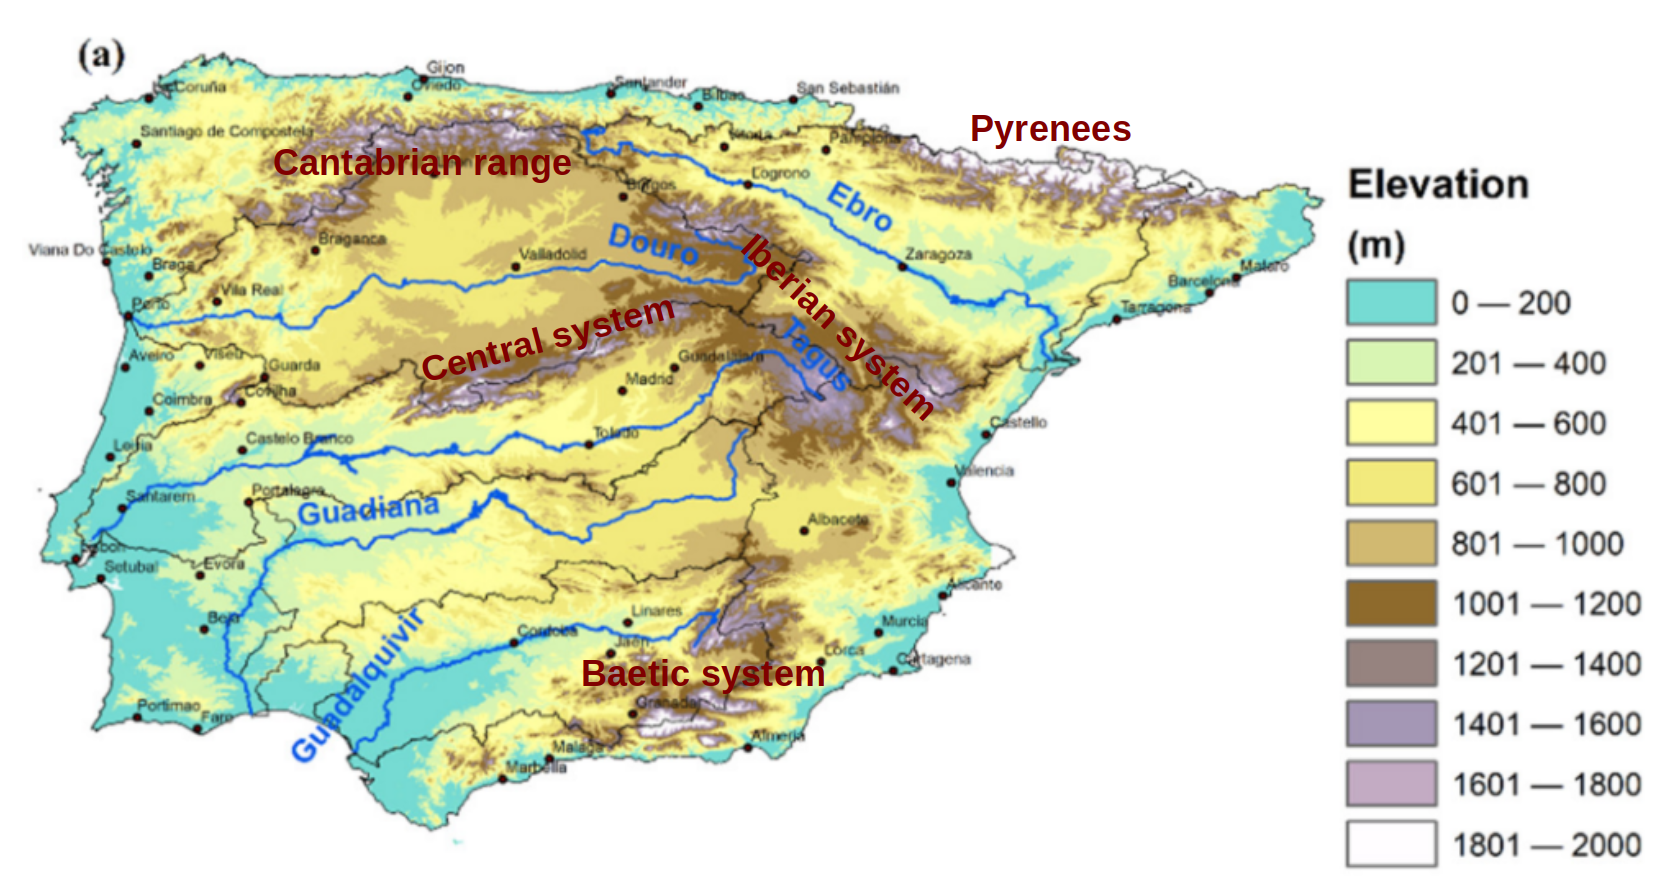
\includegraphics[width=\linewidth]{images/intro/ip_topography_fonseca_mountains.png}
    \end{subfigure}
    \begin{subfigure}{0.8\textwidth}
        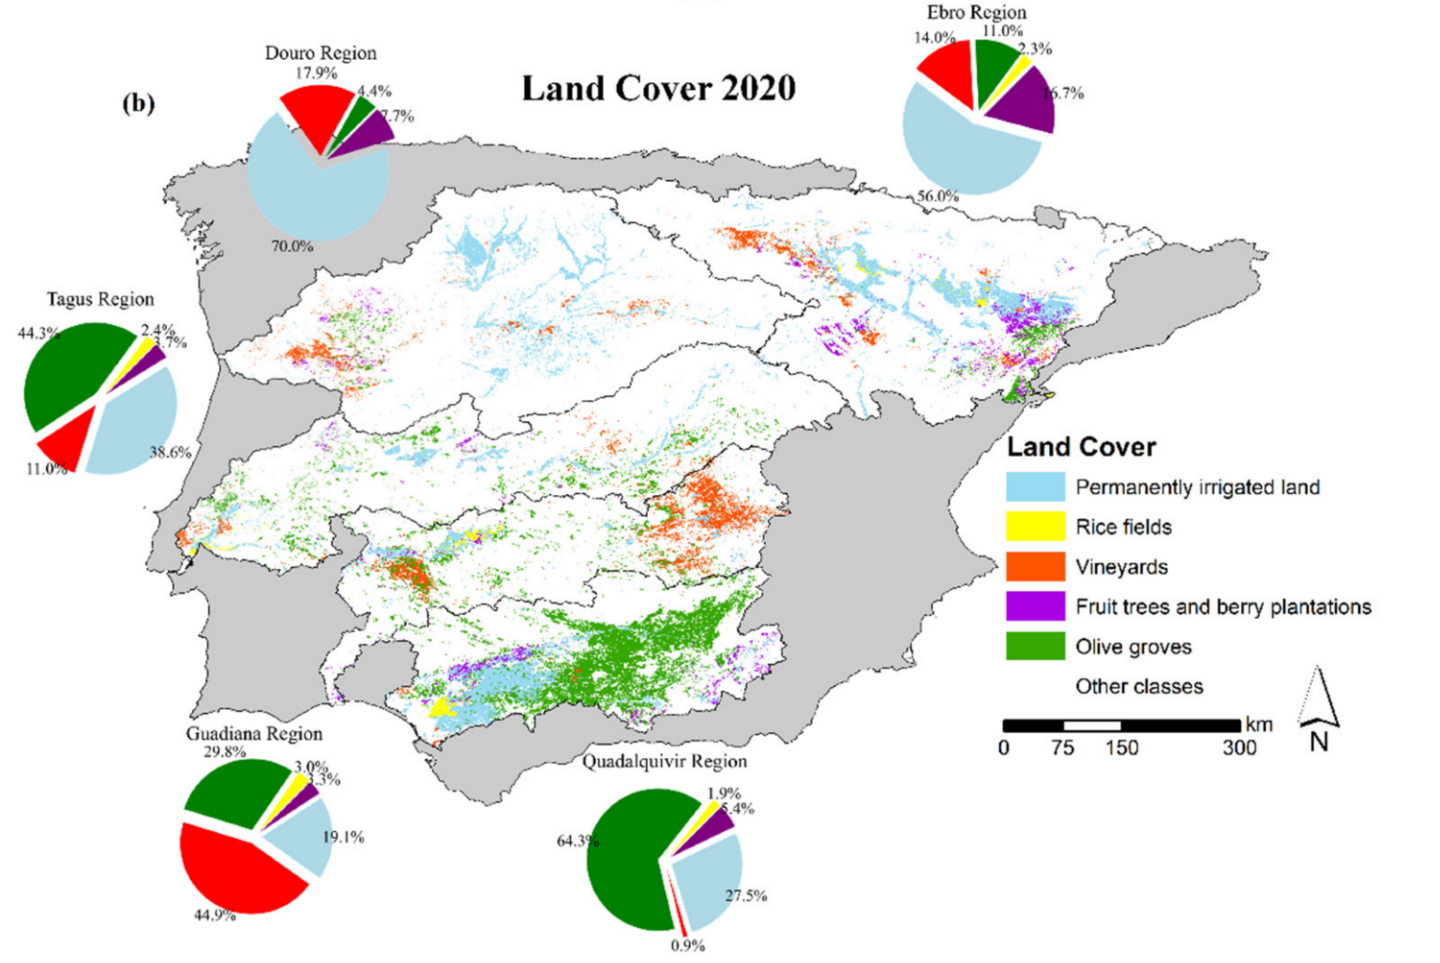
\includegraphics[width=\linewidth]{images/intro/land_cover_fonseca.png}
    \end{subfigure}
    \caption{The Iberian Peninsula: (a) topography and major rivers, (b) water-dependent land cover in major basins according to the 2020 \href{https://land.copernicus.eu/en/products/corine-land-cover}{CORINE} database. Adapted from \citet{fonseca_agricultural_2022}.}
    \label{fig:IP_map_fonseca}
\end{figure}

Irrigation has long been present in this region, as demonstrated by archeological studies of the Bronze Age \citep[2140-1500 BCE, ][]{mora-gonzalez_isotopic_2016} or in the Roman and Islamic eras \citep[250-800, ][]{butzer_irrigation_1985}. 
Nowadays, it is an essential agricultural pratice, as illustrated by the share of land covers identified as water-dependent in \citet{fonseca_agricultural_2022}, shown in Fig. \ref{fig:IP_map_fonseca}b. 
According to the \href{https://data.apps.fao.org/aquastat/?lang=en}{AQUASTAT} database \citep[presented in][]{frenken_aquastat_2012}, annual irrigation withdrawals in Spain and Portugal were estimated at 22.8 $\cdot 10^{9} m^3$ on average over the period 2010-2022.
The Ebro and Guadalquivir basins are particularly known for their intensive irrigation practices, and irrigated areas are still expanding in the 21st century, with respective increases of +40\% and 53\% between 1990 and 2020 \citep{fonseca_agricultural_2022}. A large share of these cultivated land falls into semi-arid areas like the Ebro valley ("steppe" climates in the Köppen-Geiger classification), or temperate with dry summers like the Guadalquivir valley (Fig. \ref{fig:IP_climate}a).

%peninsula climate and precip
\begin{figure}[h!]
    \centering
    \begin{subfigure}{0.8\textwidth}
        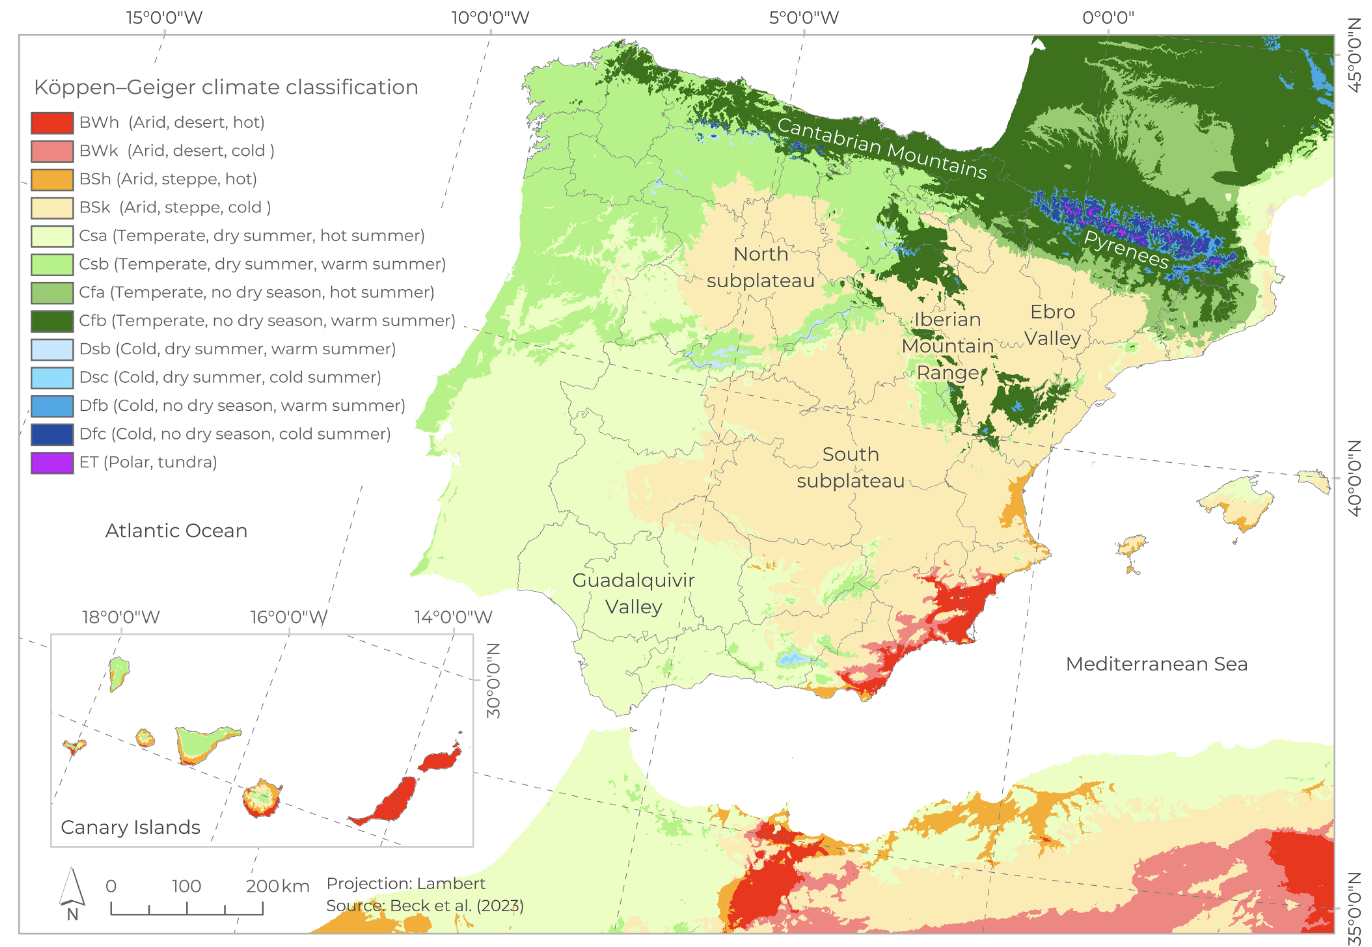
\includegraphics[width=\linewidth]{images/intro/koppen_IP_correa.png}
    \end{subfigure}
    \begin{subfigure}{0.8\textwidth}
        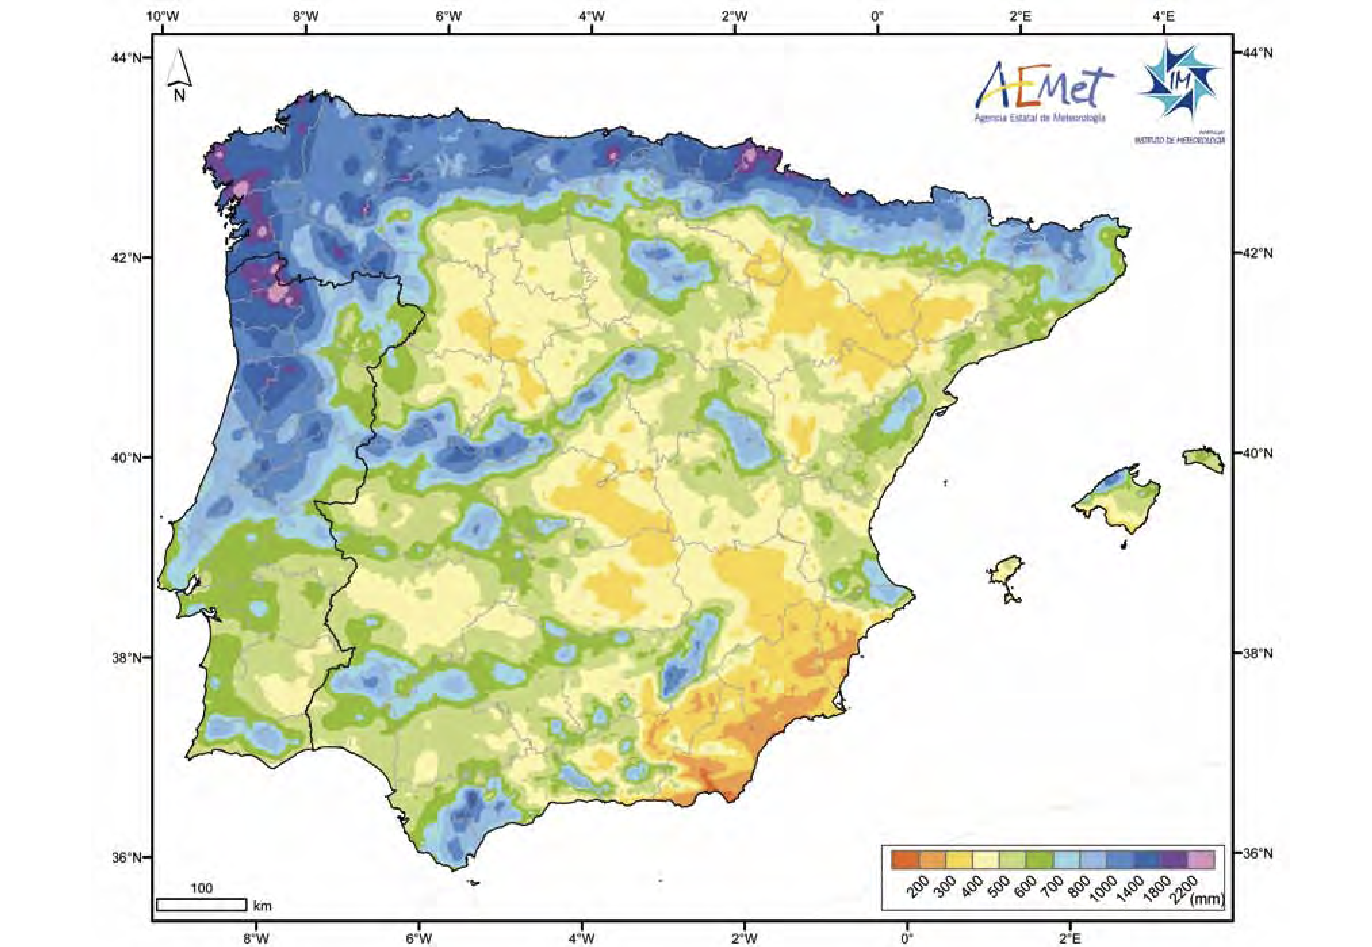
\includegraphics[width=\linewidth]{images/intro/precip_IP_1970-2000.png}
    \end{subfigure}
    \caption{(a) Köppen-Geiger classification of the Iberian Peninsula (1991-2020), taken from \citet{correa_analysis_2024} based on \citet{beck_high-resolution_2023}. (b) Annual mean precipitation (1970-2000) according to the Iberian Climate atlas \citep{cunha_atlas_2011}.}
    \label{fig:IP_climate}
\end{figure}

These climates explain the high reliance on artificial methods to sustain water supply to crops throughout the year and, depending on the regions, various infrastructures have been developed to enable irrigation. 
River dams with a wide range of reservoir sizes can store water in winter and spring when surface runoff and river discharge are high (see Fig. \ref{fig:selected_stations} and associated discussion on river dams), making it available later in the year for irrigation and other services such as hydropower generation.
According to the \citet{ICOLD2020}, there are at least 1064 dams in Spain, making it one of the top 10 dam-building countries \citep{sadki_implementation_2023}.
Mountainous areas receive most of the precipitation over the Peninsula (Fig. \ref{fig:IP_climate}b), including in the form of snow, and canals can be used to transport water to cultivated areas in the drier valleys. The Canal d'Urgell \citep{farran_urgell_2024} in the Segre sub-basin, further described in Chapter \ref{chap:liaise}, is a very good example of this type of infrastructure.
Finally, groundwater pumping is also a major water source for irrigation. It was estimated to provide water for one third of irrigated areas in Spain in \citet{de_stefano_groundwater_2015}, and its general role in freshwater supplies is still increasing \citep{llamas_groundwater_2015}. Some of these resources, particularly in the arid regions of the southeast, come from so-called \textit{fossil} aquifers, leading to the use of the term \textit{groundwater mining} when recharge takes more than 50 years \citep{custodio_groundwater_2016}.
The intensification of these practices is responsible for rapid groundwater depletion which pauses risks for the quality and future availability of water resources, raising economic and ethical concerns \citep{custodio_groundwater_2017}.

Other concerns for the sustainability of irrigation arise from ongoing and future climate change in the region. The Intergovernmental Panel on Climate Change 
\citep{RN1} identified arid and semi-arid regions, like the Mediterranean basin \citep{giorgi_climate_2006}, as very sensitive to adverse impacts of a global temperature increase, some of which are already underway and visible in observations.
This includes more frequent and intense extreme events \citep{dominguez-castro_high_2019}, but also long-term increases in temperature \citep{pena-angulo_seasonal_2021,gonzalez-hidalgo_variability_2022}. At present, the annual signal on precipitation remains uncertain, but shifts in spatial and seasonal patterns have already been identified, which could disrupt the availability of water resources over the Peninsula \citep{gonzalez-hidalgo_seasonal_2024}. 
For the future, global change scenarios generally predict a warming and decrease in precipitation over the region \citep{pereira_temperature_2021}, with associated consequences on soil moisture, evapotranspiration, and vegetation \citep{RN1, nunes_effects_2023}.
In particular, the concepts of desertification and aridification, although not unanimously defined, are being increasingly studied in the region, to analyse ongoing trends \citep{paniagua_aridity_2019, begueria_aridity_2025}, and evaluate adaptation policies \citep{van_leeuwen_evolution_2019, MITECO2022}. For instance, a shift in agricultural practices, favouring rainfed agriculture is considered essential to reduce the impacts of irrigation on regional water security \citep{eekhout_how_2024}. The ongoing shift from flood to drip irrigation was also estimated by \citet{pool_flood_2021} to have larger influence on groundwater recharge than climate change in the region of Valencia, highlighting the need for comprehensive assessments of the impacts of irrigation. Focusing on a sub-catchment of the Ebro basin which transitioned to irrigated agriculture in the 21st century, \citet{von_gunten_estimating_2015} showed increases in groundwater storage over irrigated areas, but also higher vulnerability of base flow in a changing climate, and insisted on the need to account for atmospheric feedback to enable precise projections.

For such studies, climate models are essential tools that can help gain understanding of the relationships between weather and long term trends in the water cycle and regional climate, and provide projections of the future climate. Their relevance for such purposes, however, depends on their ability to represent the complex interactions at the interface between land surfaces and the atmosphere. The next section therefore provides an overview of these physical processes and of their representation in climate models.

\clearpage

\section{Land-atmosphere interactions}
\label{sec:l-a_interactions}

Over land, interactions between the surface and the lower layers of the atmosphere have significant impacts on meteorological (air temperature and humidity, precipitation, wind) and hydrological (runoff, stream flow, soil moisture) variables. The two systems influence each other's water and energy budgets, and multiple feedback loops can be identified depending on the spatial and temporal scales considered. The complexity of this coupling and the variety of impacts it can have on ecosystems and human activities make it a subject of interest for climate science and a necessary component of climate or NWP models. This section aims to provide a state-of-the-art description of these interactions and their modelling, as well as the impacts irrigation can have on them. 

\subsection{Water and energy budgets at the surface}
To understand the components of the land-atmosphere coupling, it is necessary to recall the main fluxes of water and energy at the surface. 
Figure \ref{fig:budgets} depicts the various components of these two budgets.

\begin{figure}[ht]
    \centering
    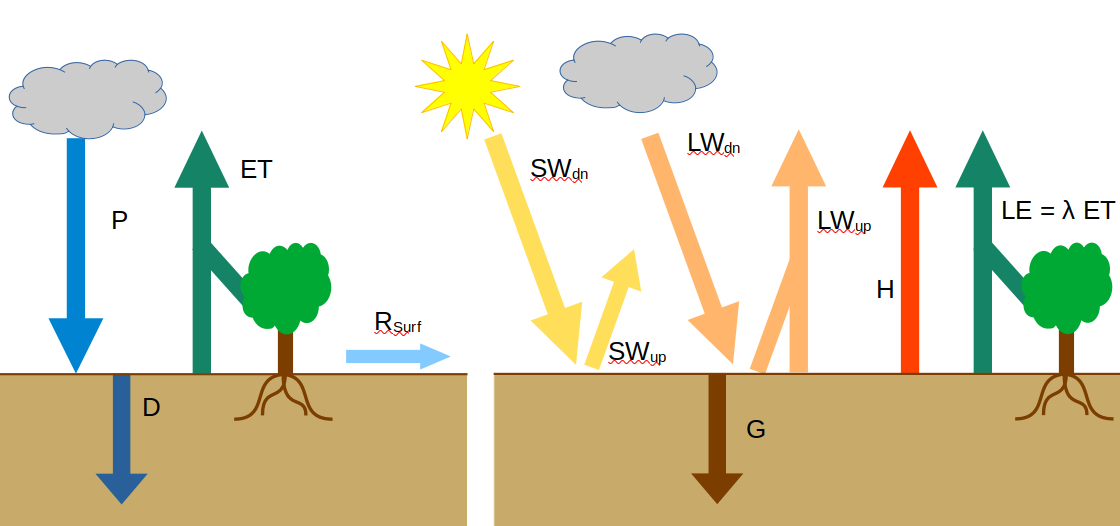
\includegraphics[width=\textwidth]{images/intro/budgets.png}
    \caption{Surface water and energy budgets. Based on similar figures from \citet{seneviratne_investigating_2010,lunel_interactions_2024}
    }
    \label{fig:budgets}
\end{figure}

The surface water budget accounts for:
\begin{itemize}
    \item \textbf{Precipitation} (transfer from the atmosphere to the surface), $P$.
    \item \textbf{Evapotranspiration} (transfer of liquid or solid water from the surface to the atmosphere in gaseous form), $ET$. It is the sum of direct evaporation and of transpiration, a process in  which vegetation releases water is has collected in the soil.
    \item \textbf{Drainage} of water in the soil to lower layers, denoted  as $D$. 
    \item \textbf{Surface runoff}, $R_{surf}$, water that does not infiltrate in the soil and flows out of the area considered.
\end{itemize}

The equation governing the evolution of water quantity in the upper soil layer (denoted here as $W_{surf}$) is:
\begin{equation}
    \frac{dW_{surf}}{dt} = P - ET - R_{surf} - D
\end{equation}

\hfill

The surface energy budget includes:
\begin{itemize}
    \item \textbf{Shortwave radiation} (SW), with an incoming term ($SW_{dn}$) corresponding to incident solar radiation and an outgoing term ($SW_{up}$) corresponding to the portion reflected by the surface.

    The difference between these two terms and the albedo of the considered surface are defined as:

    $SW_{net} = SW_{dn} - SW_{up}$

    $\alpha_{SW} = SW_{up}/SW_{dn}$.
    \item \textbf{Longwave radiation} (LW), with an incoming term ($LW_{dn}$) corresponding to the infrared radiation reflected or emitted by clouds and atmospheric gases reaching the surface and an outgoing term ($LW_{up}$) corresponding mostly to the infrared radiation emitted by the surface based on its temperature, as well as a partial reflection of the incoming LW radiation.

    The difference between these two terms is defined as $LW_{net} = LW_{dn} - LW_{up}$.
    
    The net radiation is also defined as the sum of the two radiation terms: $R_{n} = SW_{net} + LW_{net}$.
    \item \textbf{Sensible heat flux} $H$, which is a thermal energy transfer between the air and the surface.
    \item \textbf{Latent heat flux}, which corresponds to the energy used to evaporate water at the surface. This energy flux is directly related to evapotranspiration (water flux) through the enthalpy of vaporization ($\lambda$), and is therefore denoted as $LE = \lambda ET$.
    \item \textbf{Heat flux into the soil}, which is a thermal conduction transfer between the considered surface layer and the lower soil layers, denoted as $G$.
\end{itemize}

The equation governing the evolution of energy in the surface soil layer (denoted here as $E_{surf}$)  is:
\begin{equation}
    \frac{dE_{surf}}{dt} = R_{n} - G - \lambda ET - H
\end{equation}

\subsection{The atmospheric boundary layer}

In meteorology, the atmospheric boundary layer (ABL) is defined as the lower part of the troposphere directly influenced by the presence of the surface. This layer is where shallow convection and turbulent diffusion phenomena occur, contributing to energy diffusion and mixing of the air.
The height of the boundary layer varies during the diurnal cycle depending on air stability, which is related to the presence of vertical temperature and humidity gradients, and wind. It can measure a few tens of meters at night and up to a few kilometers during the day in arid regions \citep{garratt_review_1994}.

The lowest part of the boundary layer is called the \textit{surface layer}. 
In these first few tens of meters, the influence of the Coriolis force is negligible compared to that of the surface, which generates strong gradients of wind, temperature and humidity. The empirical similarity theory developed by Monin and Obukhov describes these variables in this layer \citep{monin1954osnovnye}. 
The wind speed generally follows a logarithmic profile, which starts from zero at the surface and is very dependent on the roughness of the surface and background wind.
On a sunny day, the surface layer is warmed by the soil via conductive and convective energy transfers quantified by the sensible heat flux, and moistened through evapotranspiration. The air in the surface is therefore nos stable, leading to the formation of thermal updrafts. 
These ascending motions, along with turbulent diffusion processes, contribute to the mixing of air masses above the surface layer. Most of the ABL is therfore constitutes by the \textit{mixed layer}, directly above the surface layer, which exhibits vertically homogeneous profiles of humidity, temperature (or rather of potential temperature which accounts for variations of pressure), and, to a lesser extent, of wind (Fig. \ref{fig:abl_structure}).
This layer ends when the temperature gradient is not sufficient to sustain the ascending motions of air, in the so-called \textit{entrainment layer}, which is typically characterized by a rapid increase in potential temperature, a decrease in humidity, and faster winds.
This marks the transition to the free troposphere, where the influence of surface conditions is weak in comparison to large-scale conditions.

\begin{figure}[ht]
    \centering
    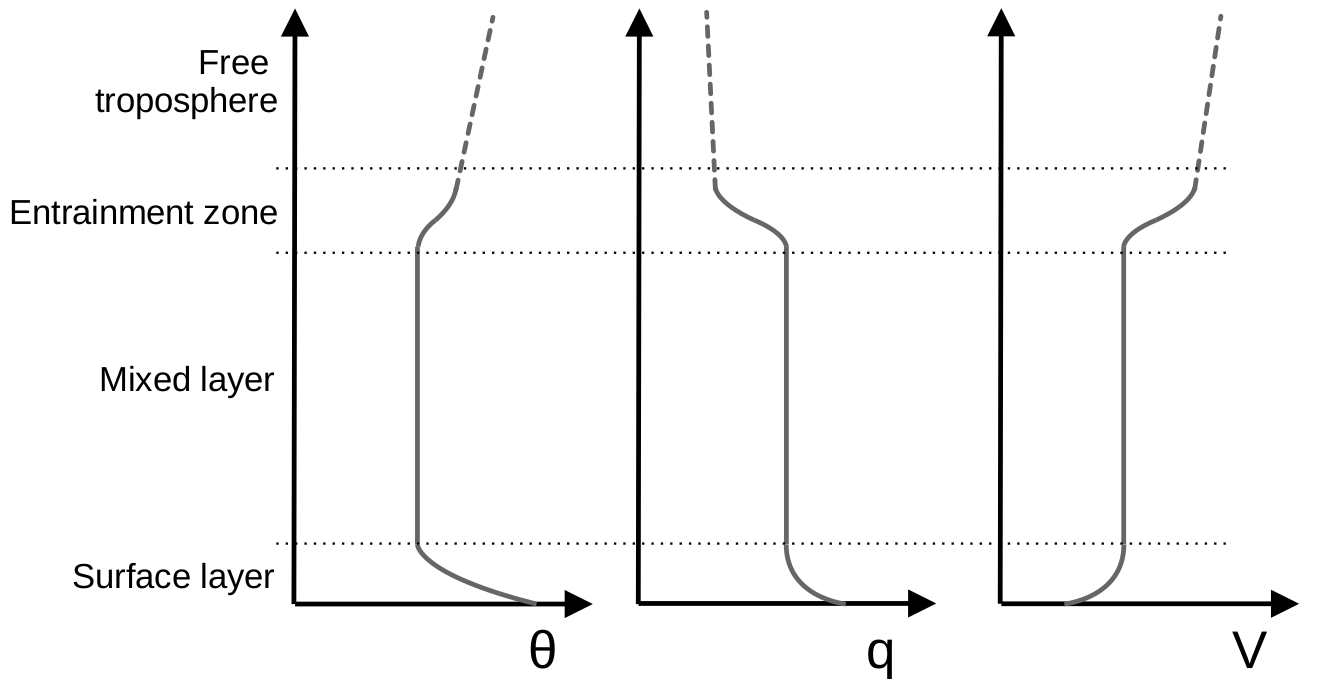
\includegraphics[width=0.7\textwidth]{images/intro/abl_lunel.png}
    \caption{Typical vertical profiles of potential temperature($\theta$), specific humidity ($q$) and wind speed ($V$) on a clearsky day. Taken from \citet{lunel_interactions_2024}, based on \citet{stull2012introduction}.}
    \label{fig:abl_structure}
\end{figure}

The partitionning of energy between the two turbulent fluxes at the surface ($\lambda ET$ and $H$) plays an essential role in the development of the boundary layer. As a tought experiment, for a given net radiation $R_n$ and a nearly constant soil heat flux (e.g., over 24 hours if there is equilibrium between daytime and nighttime), the remaining energy is distributed between the two turbulent fluxes. The evaporative fraction (defined here as $EF = \frac{\lambda ET}{\lambda ET+H}$, although $EF = \frac{\lambda ET}{R_n}$ is sometimes used) and the Bowen ratio (defined as $B = \frac{H}{\lambda ET}$) quantify this partitionning. If the latent heat flux is very high compared to the sensible heat flux (high $EF$, low $B$), the air temperature in the surface layer remains low because the energy is primarily used for evapotranspiration, and the soil transfers little heat to the air. Conversely, if the Bowen ratio is high, a larger portion of the incident energy is transmitted directly to the air, leading to a higher air temperature near the surface and more pronounced development of the boundary layer \citep{betts_fife_1995}.
In reality, the processes are a bit more complex since the surface temperature (and therefore the $LW_{up}$ flux) may also react to changes in latent heat flux, but the reciprocal behaviour of the latent and sensible heat fluxes has been identified in multiple observations and modelling experiments \citep{betts_fife_1995, seneviratne_investigating_2010}.

Moreover, the thermal properties of the soil are also affected by SM, as wet soil has greater thermal inertia than dry soil. In contexts where the latent heat flux is limited, this can significantly impact air temperature by affecting nighttime cooling \citep{ait-mesbah_role_2015}. The absence of solar radiation at night usually leads to radiative cooling of the soil and air in the surface layer. However, for wetter soil, this cooling will be less pronounced due to higher thermal inertia. During daytime, the impact of this inertia is often negligible, and other processes dominate the evolution of air temperature. Still, on a daily average, an increase in soil moisture can lead to an increase in air temperature since nighttime cooling is less significant \citep{cheruy_role_2017}.


\begin{figure}[ht]
    \centering
    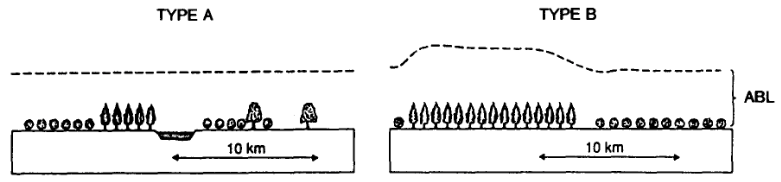
\includegraphics[width=0.9\textwidth]{images/intro/abl_heterog_garratt.png}
    \caption{Schematized ABL behaviour over two types of land surfaces. In type A, the surface structure is disorganised at length scales of 10 km or less; in type B, there is organisation at length scales greater than 10 km. Taken from \citet{garratt_review_1994}.}
    \label{fig:abl_heterog}
\end{figure}

The presence of surface heterogeneities, including those created by human activities like urban areas and cultivated land, can affect the structure of the ABL in a wide range of ways that might never be fully understood or modelled \citep{bou-zeid_persistent_2020}. 
The review by \citet{garratt_review_1994} already mentionned the importance of their organisation (Fig. \ref{fig:abl_heterog}), and identified 10 km as a threshold length scale to observe different ABL structures over heterogeneous terrain. 
More recently, \citet{bou-zeid_persistent_2020} distinguished four classes of heterogeneities, semi-inifinite interfaces with a single transition between two large surfaces (<100 km), large individual patches (cities or lakes), repeating patterns of small patches, and unstructured heterogeneities. 
The large contrasts in the first and second case can initiate specific winds, like sea and lake breeze circulations \citep{crosman_sea_2010,kenny_numerical_2017}, and similar phenomena at the transition between cities and rural landscape \citep{hidalgo_urban-breeze_2008,omidvar_plume_2020} or along large rivers \citep{zhang_large-eddy_2023}. In the third catergory, when heterogeneous patches are smaller than the ABL characteristic height, it is often possible to assume that differences are limited to the surface layer but disappear in the mixed layer, as shown for type A in Fig. \ref{fig:abl_heterog}. The fourth type of heterogeneities, although most common, is still poorly understood and accounted for in models.
In all these cases, the strength and direction of the ambient wind is essential, affecting advection terms, and the presence of internal boundary layers or secondary circulations \citep{anderson_turbulent_2020, zhang_large-eddy_2023}. 
For models, LES experiments allowed to identify blending heights above heterogeneous surfaces and develop mesoscale parametrizations, initially focusing on variations of surface roughness \citep{bou-zeid_large-eddy_2004}, then on surface temperature and turbulent fluxes \citep{stoll_surface_2009}. Approaches to account for the diversity of surface fluxes were then introduced in coarser models \citep{ament_improved_2006}. Studying soil moisture heterogeneities in California in NWP models, \citet{alexander_simulating_2022} found that the choice in LSMs dominated variations in the response of the ABL, rather than the parameterization of turbulence, confirming previous findings that soil moisture and subsurface conditions strongly affect ABL development throughout the day \citep{rihani_isolating_2015}.

\subsection{Role of soil moisture in land-atmosphere interactions}

The term \textit{coupling} between the surface and the atmosphere encompasses multiple influences and feedbacks between the two systems. Soil moisture (SM) plays a central role in this coupling through its direct and indirect interactions with evapotranspiration, precipitation, and the surface energy budget.

\subsubsection*{Coupling between soil moisture and evapotranspiration}

Soil moisture is a key factor in the description of evapotranspiration regimes initially established by \citet{Budyko_1956, Budyko_1974}. Three main regimes are identified for the evolution of the evaporative fraction $EF$. Figure \ref{fig:evap_regimes} represents these regimes.

\begin{itemize}
    \item If soil moisture is below a threshold $\theta_{WILT}$, called the wilting point, plants cannot extract water to transpire, bare soil no longer evaporates, and evapotranspiration (and thus the evaporative fraction) is zero. This first regime is called the \textbf{dry regime}.
    \item If soil moisture is above a critical threshold $\theta_{CRIT}$, soil moisture has no impact on $EF$, which is maximal. Evaporation is limited by the available incident energy, it is the \textbf{wet regime}.
    \item Between $\theta_{WILT}$ and $\theta_{CRIT}$, there is a \textbf{transition regime} where evapotranspiration is primarily conditioned by soil moisture. 
\end{itemize}

\begin{figure}[ht]
    \centering
    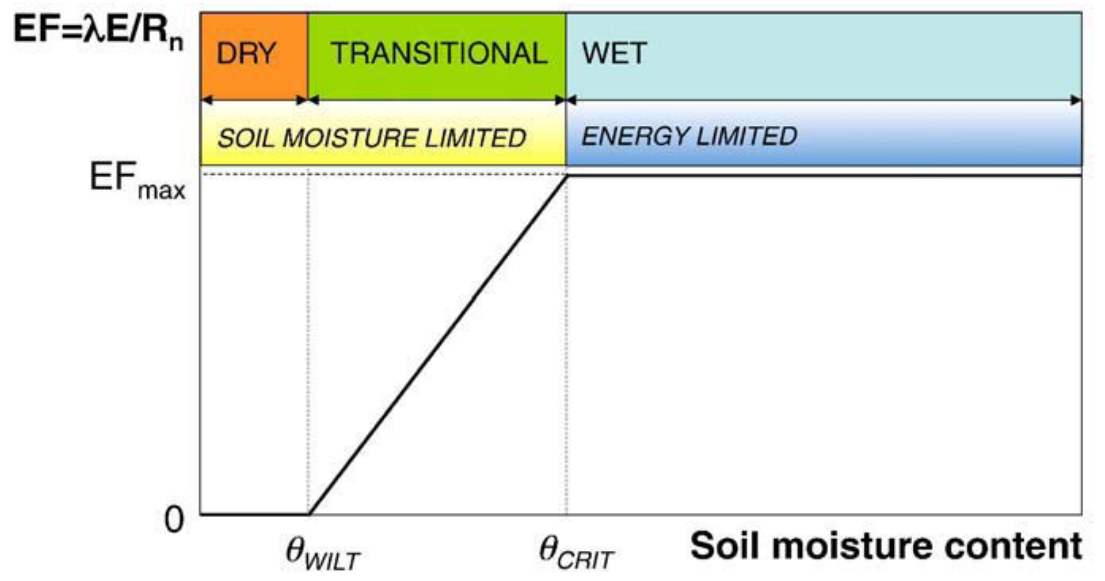
\includegraphics[width=0.7\textwidth]{images/intro/evap_regimes.png}
    \caption{Representation of different evapotranspiration regimes. Taken from \citet{seneviratne_investigating_2010}.}
    \label{fig:evap_regimes}
\end{figure}

Through its influence on evapotranspiration, soil moisture directly impacts surface water and energy budgets, particularly the distribution of energy between turbulent fluxes. As explained earlier, this has consequences for air temperature and humidity in the boundary layer.

However, there are also several the feedbacks of evapotranspiration on soil moisture. First, an increase in evapotranspiration directly leads to a decrease in soil moisture and an increase in air humidity. This contributes to reducing the vertical humidity gradient between the air and the surface, which tends to limit evaporation \citep{allen_crop_2000}, forming a negative feedback loop. It is also established that an increase in air temperature leads to higher evaporative demand \citep{jarvis_stomatal_1986}. If enough water is available in the soil, a temperature increase will increase evapotranspiration, thus decreasing soil moisture. This can form a positive feedback loop where dry soil leads to high air temperatures, resulting in even drier soil and possibly initiating extreme drought events \citep{quesada_asymmetric_2012}. If no more water is available or if there are no more gradients between the soil surface and the air, the influence of air temperature on soil moisture becomes neutral, and the feedback loop is interrupted.

\subsubsection*{Coupling between soil moisture and precipitation}

The most complex processes of surface-atmosphere coupling concern the link between soil moisture and precipitation. Several opposing effects are at play, with a large importance of spatial heterogeneities of soil moisture at the surface, which may derive from the diversity of vegetation, soil types, orographic features, and anthropogenic processes like irrigation.

Increases in SM and ET have been associated with direct increases in precipitation in both modelling and observational studies \citep{koster_observational_2003, guo_glace_2006, wei_dissecting_2012, findell_probability_2011}, constituting a positive feedback loop \citep[moisture recycling, as presented in ][]{eltahir_precipitation_1996}.
However, high soil moisture can lead to a stabilisation of the boundary layer by reducing the sensible heat flux.
This stabilisation inhibits vertical development and convective processes involved in cloud formation and precipitation \citep{findell_atmospheric_2003-1, ek_influence_2004}. 
This constitutes a negative feedback loop where convective rainfall is more likely to occur over drier soil patches, which was noticed in observations \citep{taylor_afternoon_2012, klein_dry_2020}. These findings suggest that indirect processes related to boundary layer structure and heterogeneities can locally exceed the direct process of atmospheric moisture recycling, although demonstrating causality in such observational studies remains challenging \citep{salvucci_investigating_2002, guillod_land-surface_2014}. Building on the purely spatial analysis of \citet{taylor_afternoon_2012}, a spatiotemporal analysis of correlations between soil moisture and precipitation highlighted the importance of temporal variability \citep{guillod_reconciling_2015}. It showed that while precipitation is more frequently triggered over drier areas, it occurs on days that are wetter relative to the season and region concerned.
Finally, spatial heterogeneities in soil moisture have also been identified as factors influencing precipitation through mesoscale circulations that can either favour or inhibit convection triggering \citep{findell_atmospheric_2003, taylor_frequency_2011, rochetin_morphology_2017}.

\subsection{Land-atmosphere interactions in climate models}

In modern ESMs or NWP models, the modelling of land-atmosphere interactions involves both the atmospheric model and the land surface model, and the modelling choices for their coupling.
From the perspective of an atmospheric model, latent and sensible heat fluxes at the surface constitute necessary boundary conditions for solving turbulent diffusion equations throughout the considered atmospheric column. These conditions impact essential meteorological variables such as air temperature, wind, and humidity. From the perspective of the LSM, precipitation computed in the atmospheric model constitutes a water input for the soil column, while surface layer characteristics (humidity, temperature, wind) condition evapotranspiration demand.

Various experiments have been designed to quantify the importance of surface coupling processes for atmospheric models. In particular, the GLACE experiments \citep{koster_glace_2006} compared atmospheric simulations with different prescribed soil moisture conditions to isolate the influence of soil moisture on precipitation. This led to the identification of hotspots: regions where this coupling is particularly pronounced. These are mainly semi-arid regions (Sahel, Great Plains in the USA) where the transitional evaporation regime described in Figure \ref{fig:evap_regimes} is more frequent than dry and wet regimes \citep{koster_regions_2004}.
This was confirmed by other modelling studies that also identified various mechanisms through which land surface conditions can impact the atmosphere in these coupling hotspots, and metrics to quantify them \citep{dirmeyer_terrestrial_2011,santanello_landatmosphere_2018, zou_precipitation_2023}.
The GLACE-CMIP5 experiments \citep{seneviratne_impact_2013} extended these conclusions by highlighting the importance of this coupling in the global warming response observed in these hotspots \citep{berg_interannual_2015}.
\citet{dirmeyer_intensified_2014} also found that the controls exterted by the land surface on boundary layer development would strengthen under climate chance, amplifying the sensibility to land use change and climate extremes in these hotspots.
More recent anlyses confirmed that the mean climate simulated by current ESMs is still highly dependent of land processes, particularly evapotranspiration \citep{zarakas_land_2024}, and of the atmospheric feedbacks they induce \citep{lague_separating_2019}.

\hfill

A particular challenge in modelling this coupling within an ESM arises from the size of the grid cells used (generally around 100 km for long climate simulations). At this scale, numerous subgrid heterogeneities exist at the surface, requiring the aggregation and averaging of highly diverse land-atmosphere interactions depending on vegetation cover, elevation, or anthropogenic factors (cities, irrigation).

For example, regarding the triggering of convective rainfall in heterogeneous areas, \citet{moon_soil_2019} showed that CMIP5 models correctly reproduced the positive temporal feedbacks (rain on wetter days) described in \citet{guillod_reconciling_2015} but not the negative spatial feedbacks identified in \citet{taylor_afternoon_2012}. The influence of resolution and parametrization choices (especially for deep convection) on the importance of land-atmosphere coupling in models has also been highlighted by \citet{tuinenburg_high-resolution_2020} and \citet{lee_weaker_2024}.

The association of observations and different scales of modelling help to document the impact of these heterogeneities and explore better ways to account for them in models. For instance, the  Models and Observations for Surface-Atmosphere Interactions (MOSAI, \cite{lohou_model_2022}) project relies on measurement campaigns specifically dedicated to studying land-atmosphere interactions in heterogeneous land cover and aims at comparing multiple models with these observations. In August 2023, I had the opportunity to take part to one of the three special observation periods of the MOSAI project in Lannemezan, although it was not in the scope of my PhD thesis to work with data from this project.

\hfill

It is now well known that accurately representing surface-atmosphere couplings is essential for accurately representing climate, particularly temperature and precipitation extremes \citep{jaeger_impact_2011, van_den_hurk_acceleration_2011}. Furthermore, the study of CMIP5 simulations has revealed a warm bias in most models, particularly in the Mediterranean basin \citep{christensen_temperature_2012, mueller_systematic_2014}. By comparing CMIP5 model biases with satellite observations, \citet{al-yaari_satellite-based_2019} also showed that these temperature biases are correlated with soil moisture biases. More generally, surface interaction processes have been identified as a crucial factor in the appearance of these biases, especially the partitioning of energy between latent and sensible heat fluxes and the underestimation of evapotranspiration \citep{cheruy_combined_2013, cheruy_role_2014,williams_land-atmosphere_2016,ma_causes_2018}. 

New developments were carried out in climate models between CMIP5 and CMIP6 \citep[e.g.][]{lawrence_community_2019, cheruy_improved_2020}, but there are still few publications analysing the CMIP6 simulations regarding land-atmosphere processes. Improvements and better inter-model agreement have been noted for surface radiative fluxes \citep{wild_global_2020} and for energy and water fluxes in general except for the Amazon, the Tibetan Plateau, and with limitations for turbulent fluxes in dry regions \citep{li_evaluation_2021}. The CMIP6 ensemble is found to perform better than any single model for evapotranspiration, which remains generally overestimated over continents, as well as evaporative fractions \citep{wang_evaluation_2021, yuan_understanding_2022}.
Regional analyses found improvements in the representation of precipitation and soil moisture over the USA \citep{srivastava_evaluation_2020, yuan_historical_2021}, but excessive land-atmosphere coupling strength in East and Southern Africa \citep{mwanthi_representation_2024}. A comparison of the CMIP6 ensemble to the ERA5 reanalysis and observation data showed that a warm bias is still present in Southern Europe although mostly decorrelated from soil moisture biases \citep{osso_assessment_2023}. 
Substantial model uncertainty on land-surface conditions still remains in CMIP6 models \citep{yuan_historical_2021}, and the importance of land-use and land-cover representation to properly represent surface energy partitioning and precipitation has been renewed for this generation of climate models \citep{devanand_land_2020,singh_land-use_2024}, justifying efforts to account for agricultural practices like irrigation.

\subsection{Impacts of irrigation on land-atmosphere interactions}
\label{sec:irrig_landatmosphere}
Human activities can influence the various components of land-atmosphere coupling. This is particularly the case with irrigation, which directly modifies soil moisture through artificial water inputs and can create strong spatial heterogeneities. 

\subsubsection*{Observations and high resolution modelling}

Observational studies have established that irrigation leads to a moister and cooler atmosphere near the surface \citep{bonfils_empirical_2007, mcdermid_irrigation_2023}, which is explained by an increase in the latent heat flux and a decrease in the sensible heat flux in irrigated areas \citep{rappin_landatmosphere_2022, boone_land_2025}.
Based on observation records in California, \citet{bonfils_empirical_2007} estimated a decrease of 1.8 to 3°C in the average summer temperature since the development of irrigation practices. This cooling effect can limit temperature values during extreme meteorological events \citep{thiery_present-day_2017, thiery_warming_2020}. However, the cooling due to increased latent heat flux can be partially compensated on a daily scale by a weakening of nighttime cooling due to thermal inertia \citep{chen_irrigation_2018}.
In the American Midwest, \cite{nocco_observation_2019} showed that the coupling effects could impact the regional climate and even mask the rise in temperature induced by global warming. Different regional responses of precipitation have also been observed, such as a decrease in irrigated areas \citep{alter_rainfall_2015} or an increase in downwind regions \citep{deangelis_evidence_2010}.
The other impacts on the atmosphere (structure of the boundary layer, mesoscale circulations, precipitation) are more complex to characterize because they do not always occur solely over the irrigated area.

\hfill

To get more insights than what point-based or satellite observations provide and analyse the atmospheric processes involved, mesoscale modelling studies have often been used to complement observational campaigns. 
The Great Plains irrigation experiment \citep[GRAINEX,][]{rappin_great_2021} measurements and simulations with the Weather Research and Forecasting (WRF) model revealed a lower ABL over irrigated areas, which is sustained throughout the growing season independently of background atmospheric conditions \citep{lachenmeier_irrigated_2024}, and a reduction of existing mesoscale slope-induced circulations in the presence of irrigation \citep{rappin_landatmosphere_2022, phillips_influence_2022}. Computing land-atmosphere coupling metrics from observation data, irrigated fields were found to be more favourable to convection than non-irrigated ones in the day \citep{whitesel_assessing_2024}. In modelling experiments over the GRAINEX study area, the choice of the irrigation fraction map and its resolution were identified as important drivers of land-atmosphere interactions \citep{lawston-parker_investigating_2023}. This study attributed it to the importance of boundaries between irrigated and non-irrigated zones, and emphasized the need to account for soil moisture heterogeneities induced by irrigation.
In the Ebro Valley (northern Spain), Meso-NH simulations at 2-kilometer and 400-meter resolution were conducted over the area of the Land Surface Interactions with the Atmosphere over the Iberian Semi-Arid Environment campaign \citep[LIAISE, ][, which will be further presented in Chapter \ref{chap:liaise}]{boone_land_2019}. They reproduced the observed differences between irrigated areas and neighboring areas in turbulent fluxes and air temperature and were greatly improved by representing irrigation \citep{lunel_irrigation_2024}. They also highlighted a weakening of the regional sea-breeze regime due to irrigation, which reduces the pressure gradient force \citep{lunel_marinada_2024}.  

Multiple mesoscale modelling studies were also conducted without being associated to specific observation campaigns, particularly with the WRF atmospheric model and the Noah LSM, showing that the representation of irrigation improves model performance, especially limiting warm biases \citep{qian_modeling_2013, yang_impact_2017,qian_neglecting_2020, liu_simulating_2021}. Over the American Great Plains, they identified a lowering of the boundary layer and lifting condensation level \citep{qian_modeling_2013}, and a reduction of the summertime precipitation deficit by increasing the frequency of mesoscale convective systems \citep{qian_neglecting_2020}. In the Colorado River basin, \citet{yang_impact_2017} showed an increase in precipitation linked to irrigation due to moisture recycling over the Sierra Nevada mountains. This positive feedback loop and strengthening of the water cycle at the basin scale had also been described in simulations using the global Community Atmosphere Model (CAM) coupled with the Community Land Model (CLM) to study the local and remote impacts of irrigation in California's Central Valley \citep{lo_irrigation_2013}. 
Similar processes of regional precipitation recycling were identified by \citet{zhang_us_2025} in the US Corn Belt region with a larger impact on drier years.
Conversely, a negative feedback loop on precipitation in Saudi Arabia was described in \citep{lo_intense_2021}, with moisture convergence leading to increased precipitation in a remote area west of the irrigated region. Very heterogeneous effects on simulated precipitation were also found in China \citep{liu_simulating_2021}, where the importance of indirect effects on climate through vegetation greening was also identified \citep{liu_irrigation-induced_2023}. In the Po valley in Italy, convection-resolving simulations over the summer 2015 found that irrigation prevented a drying of the soil during a heatwave, moistened the air and limited warming by 2.5-3K \citep{valmassoi_regional_2020}. This impact propagated to the boundary layer, which was lowered from 1500 to 1000 m but did not lead to any no precipitation feedback.

These results were obtained with very diverse representations of irrigation since not all models target the same objectives. For example, the experiments with WRF-Noah or Meso-NH-SURFEX \citep{lunel_irrigation_2024} used idealized representations that maintain SM at field capacity in irrigated areas to limit stress for the vegetation. This type of modelling is suitable for short simulations over a limited domain but for Earth System Models (ESMs), water-conservative approaches are necessary to run long-term global simulations while keeping a consistent water cycle representation \citep{valmassoi_review_2022}. 

\subsubsection*{Impacts of irrigation in ESMs}

The impacts of irrigation on specific regions have been studied for several decades, but interest in its impacts on global climate is more recent \citep{boucher_direct_2004}. By comparing coupled simulations with and without irrigation, \citet{sacks_effects_2009} found no influence on the global mean temperature but small regional cooling (less than 1 K) at mid-latitudes. 
In more recent studies, LSMs that represent irrigation were shown to represent the shift in energy partitioning between the turbulent fluxes, achieving large increases in latent heat flux \citep{pokhrel_incorporating_2012, al-yaari_role_2022, arboleda-obando_validation_2024}. 
Irrigation modelling was found to induce a cooling on yearly average values, with seasonal and regional impacts that remain highly varied \citep{puma_effects_2010, cook_irrigation_2015}. 
In general, regional effects within global simulations are mostly visible and analysed in irrigation hotspots such as India, Eastern China and the USA, although \citet{chen_global_2019} pointed that the Community Earth System Model \citep[CESM, ][]{danabasoglu_community_2020} tends to exacerbate the effects in these regions of strong surface-atmosphere coupling compared to observations. 
Using coupled simulations, \citet{cook_divergent_2020} concluded that even under a strong climate change scenario, irrigation would keep moderating warming and drying but warned that for regions like Mexico and the Eastern Mediterranean, ``current irrigation rates will be unable to compensate for expected moisture losses by the end of the 21st century, meaning that any irrigation benefit will be temporary".
According to \citet{de_vrese_uncertainties_2018}, uncertainties on the impacts of irrigation on climate can still stem from modelling choices at the interface between LSMs and GCMs. 
This study found that aggregating all surface fluxes in the LSM could limit or even reverse the moistening impact of irrigation on the atmosphere.
To limit uncertainties on the impact of irrigation on climate and the water cycle, \citet{de_vrese_uncertainties_2018, cook_divergent_2020} also both highlighted the importance of accounting for available resources and methods for irrigation withdrawals, which is not represented in all models.

Indeed, using water-conservative representations of irrigation also allows the study of the continental water cycle as a whole, accounting for impacts of irrigation withdrawals, on the conditions that they are not overly simplified by removing seawater as done in the CESM. More elaborate models can now differentiate between irrigation methods, withdrawals from surface or groundwater ressources and represent storage and adduction, offering an integrated vision of the anthropized water cycle \citep{decharme_simple_2025}.
For instance, \citet{leng_significant_2017} showed that the responses in groundwater levels and river flows to irrigation were very contrasted and highly dependent on the irrigation methods and sources used. \citet{yao_implementation_2022} confirmed these findings, and also showed that representing distinct irrigation methods in CLM improved the agreement with surface fluxes measurements.
Using global simulations, \citet{costantini_projected_2023} identified regions where the impact of climate change could limit future withdrawals, and estimated that at least 27\% of the world population would be exposed to water scarcity issues by 2100.
\citet{arboleda-obando_joint_2025} conducted a global study of the impacts of irrigation under climate change with coupled simulations, identifying more intense depletion in irrigated zones, but also atmospheric feedbacks that could increase precipitation in their non-irigated surroundings. This study projects that irrigation will be limited by future hydroclimate conditions or contribute to an increase in tensions over water use over one third of irrigated areas, including the Mediterranean basin.

Finally, global simulations allow the study of very remote connection and long term patterns. \citet{de_vrese_asian_2016} highlighted a link between irrigation in Asia and increased precipitation in East Africa, while \citet{wei_where_2013} identified moisture-importing and -exporting regions at the global scale. Running 30-years simulations with and without irrigation, \citet{guimberteau_global_2012} studied the temporal disruptions of seasonal phenomena, and identified a delay in the onset of the Indian summer monsoon due to regional irrigation effects.

\hfill

It is important to note that most ESMs participating in CMIP6 did not include irrigation modelling. In heavily irrigated regions, models representing irrigation show different historical trends in several essential climate variables (soil moisture, latent heat flux) that better match satellite observations \citep{al-yaari_role_2022}. 
Regarding the IPSL-CM used in this thesis, \citet{mizuochi_multi-variable_2020} found that in its CMIP6 simulations, the absence of irrigation was a major source of error, on soil moisture and evapotranspiration, which was amplified and propagated to errors in precipitation in coupled configuration, owing to atmospheric feedbacks.
The IRRMIP intercomparison project is designed to study in detail the various impacts of irrigation representation in ESMs to better understand the uncertainty of responses to this modelling \citep{yao_irrigation-expansion-induced_2023}. So far, the first results of this multi-model analysis have confirmed that irrigation expansion contributes to a rapid increase in withrawals and to a cooling of near-surface temperatures \citep{yao_impacts_2025}. It was also associated to less frequent heat extremes in irrigated regions, although the concurrent moistening increases the exposure of local populations to moist-heat stress \citep{yao_impacts_2025-1}.

\section{Scientific questions and thesis outline}

This chapter has shown that land-atmosphere coupling processes are a major element of the climate system and of climate models that intend to simulate it. 
Their high influence on near-surface variables and precipitation that directly affect human and animal populations and vegetation already make them a relevant object of study. This interest is strengthened by the uncertainties still associated to their representation and by the impact they can have on the results of current or future climate simulations. 
In this context, irrigation, a widespread agricultural practice that is bound to keep expanding in the future, can alter natural balances of the water and energy budgets.
Withdrawals from surface and groundwater resources disrupt the continental water cycle, and soil moisture is also directly modified by irrigation, possibly affecting land-atmosphere feedback processes.
This justifies the increasing interest in including a representation of irrigation in LSMs, to improve model performance and provide relevant predictions of the impacts of climate change in intensely irrigated regions.

Although there are exception, two main types of modelling studies can be distinguished in the literature, which both have their limitations.
On the one hand, climate modelling studies often focus on global average impacts of irrigation on climate and do not dwelve into details on the intermediary processes affected by irrigation such as the structure of the ABL, partly due to the lack of high frequency outputs \citep{findell_accurate_2024}. Their coarse resolution also often limits the analysis of regional impacts to the most intensely irrigated regions such as southern Asia or the USA, and does not enable a discussion of subgrid heterogeneities induced by irrigation. Also, since coupled simulation with a GCM are costly, they are sometimes conducted with a standalone LSM which keeps them from analysing atmospheric feedbacks, including on irrigation demand.
On the other hand, higher-resolution simulations with mesoscale (possibly cloud-resolving) models can very precisely describe local impacts of irrigation on near-surface conditions and the ABL and be compared to observation campaigns. However, their descriptions of irrigation are often idealised and tailor-made to represent local surface conditions, and do not enable an analysis of the full water cycle. Furthermore, they are often run for a few days or weeks only, which means they are not suited to study impacts on climatic time-scales.

This PhD work therefore aims to analyse the regional impacts of irrigation on climate, on both continental and atmospheric components of the water cycle, and on the atmospheric boundary layer at the diurnal scale.
It leverages a new limited area model (LAM) configuration developed for the Institut Pierre-Simon Laplace climate model (IPSL-CM) to perform simulations with the atmospheric and land surface components of the global model, ICOLMDZ and ORCHIDEE.
This regional climate model, called ICOLMDZOR LAM, can provide insight on the parametrizations of the global IPSL-CM while running with a higher resolution and lower computational costs than in global applications.

Until now, a large share of irrigation modelling studies have focused on the USA (and to some extent eastern China and southern Asia), and hinted that further research in different contexts was required to strengthen their conclusions, especially on atmospheric feedbacks which can be very dependent on mesoscale patterns.
This study focuses on the Iberian Peninsula, which does not present irrigated surfaces as large as these regions but remains a hotspot for irrigation in Europe, with major concerns regarding its sustainability in a changing climate.
Although it was not identified by \cite{koster_regions_2004} as a region of strong surface-atmosphere coupling (probably owing to its small size relative to the resolution of the model used and to other identified hotspots), its semi-arid climate is expected to make land surface-atmosphere coupling processes very sensitive to the disruptions induced by irrigation.

\hfill

Using regional climate simulations over this region, this thesis addresses the following questions:

\begin{itemize}
    \item Does simulated irrigation contribute to a better representation of the water cycle (river discharge, evapotranspiration and precipitation) over the Iberian Peninsula ?
    \item How does irrigation affect the continental water budget and atmospheric moisture recycling over the Iberian Peninsula ?
    \item What are the impacts of irrigation on land-atmosphere coupling processes and the ABL in a regional climate model ?
    \item How can a climate model be compared to punctual observation data and cloud-resolving simulations in a region of high surface heterogeneities ?
    \item What are the limitations and perspectives for improvement of the ICOLMZOR LAM in simulating the climate of the Iberian Peninsula and the impacts of irrigation in this region ? 
\end{itemize}

Chapter \ref{chap:methods} describes the components of the ICOLMDZOR LAM and the simulation setups used in this study. 
Chapter \ref{chap:routing} presents the evaluation and parameter tuning of the river routing and irrigation scheme conducted over the Iberian Peninsula.
Chapter \ref{chap:forcing} gives some insight into the influence of the lateral boundary conditions of the LAM regarding land-atmosphere coupling variables, which was explored during Mariame Maiga's master's intership. 
Chapter \ref{chap:monthly} analyses impacts of irrigation over the Iberian Peninsula in recent climate conditions and in the second half of the century under a strong climate change scenario. 
Based on the same simulations, Chapter \ref{chap:liaise} focuses on the study area and period of the LIAISE campaign to compare the LAM to observations and a mesoscale simulation and analyse the impacts of irrigation on the ABL.
Finally, Chapter \ref{chap:conclusion} summarizes the main outcomes and perspectives of this thesis.

%fin

